\documentclass[t]{beamer}
\usetheme{Copenhagen}
\usepackage{amsmath, tikz, tkz-euclide, xcolor}
\usetkzobj{all}
\setbeamertemplate{headline}{} % remove toc from headers
\newcommand{\nl}{\newline\\}

\title{Right Triangle Trigonometry}
\author{}
\date{}

\AtBeginSection[]
{
  \begin{frame}
    \frametitle{Table of Contents}
    \tableofcontents[currentsection]
  \end{frame}
}

\begin{document}

\begin{frame}{}
    \titlepage
\end{frame}

\section{Write the Exact Ratio for the Six Trigonometric Ratios} 

\begin{frame}
In geometry class, you learned about three trigonometric ratios: sine, cosine, and tangent.  \nl 

\begin{center}
    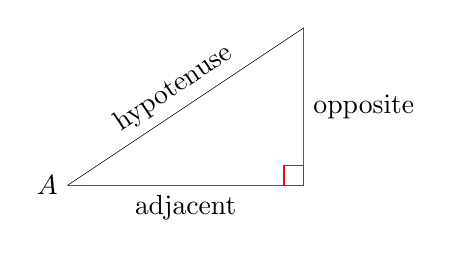
\begin{tikzpicture}
    \tkzDefPoints{0/0/A, 3/0/C, 3/2/B}
    \tkzDrawPolygon(A,B,C)
    \tkzMarkRightAngle[color=red](A,C,B)
    \tkzLabelPoints[left](A)
    \tkzLabelSegment[below](A,C){adjacent}
    \tkzLabelSegment[right](C,B){opposite}
    \tkzLabelSegment[sloped,above,midway](A,B){hypotenuse}
    \end{tikzpicture}
\end{center}
\pause
\[
\sin A = \dfrac{\text{opposite}}{\text{hypotenuse}} \hspace{0.25in} \cos A = \dfrac{\text{adjacent}}{\text{hypotenuse}} \hspace{0.25in}  \tan A = \dfrac{\text{opposite}}{\text{adjacent}}    
\]
\end{frame}

\begin{frame}{SOH-CAH-TOA}
We usually remember this as SOH-CAH-TOA.   \nl 

Sometimes you may need to use the Pythagorean Theorem, $a^2+b^2=c^2$, in order to find any missing sides.
\end{frame}

\begin{frame}{Example 1a}
Write the exact ratios for sine, cosine, and tangent of angle $A$ for each of the following.  \nl
\begin{minipage}{0.4\textwidth}
(a) \quad \nl
\begin{tikzpicture}
    \tkzDefPoints{0/0/A, 3/0/C, 3/2/B}
    \tkzDrawPolygon(A,B,C)
    \tkzMarkRightAngle[color=red](A,C,B)
    \tkzLabelPoints[left](A)
    \tkzLabelSegment[below](A,C){15}
    \tkzLabelSegment[right](C,B){8}
    \tkzLabelSegment[above,midway](A,B){17}
    \end{tikzpicture}
\end{minipage}
\begin{minipage}{0.4\textwidth}
\begin{align*}
    \onslide<2->{\sin A &= \frac{8}{17}}   \\[11pt]
    \onslide<3->{\cos A &= \frac{15}{17}}   \\[11pt]
    \onslide<4->{\tan A &= \frac{8}{15}}   \\
\end{align*}
\end{minipage}
\end{frame}

\begin{frame}{Example 1b}
\begin{minipage}{0.4\textwidth}
(b) \nl
\begin{tikzpicture}
    \tkzDefPoints{0/0/A, 3/0/C, 3/2/B}
    \tkzDrawPolygon(A,B,C)
    \tkzMarkRightAngle[color=red](A,C,B)
    \tkzLabelPoints[left](A)
    \tkzLabelSegment[below](A,C){4}
    \tkzLabelSegment[right](C,B){3}
    \tkzLabelSegment[above,midway](A,B){5}
    \end{tikzpicture}
\end{minipage}
\begin{minipage}{0.4\textwidth}
\begin{align*}
    \onslide<2->{\sin A &= \frac{3}{5}}   \\[11pt]
    \onslide<3->{\cos A &= \frac{4}{5}}   \\[11pt]
    \onslide<4->{\tan A &= \frac{3}{4}}   \\
\end{align*}
\end{minipage}
\end{frame}

\begin{frame}{Example 1c}
(c) \nl
\begin{minipage}{0.5\textwidth}
\begin{tikzpicture}
    \tkzDefPoints{0/0/A, 3/0/C, 3/2/B}
    \tkzDrawPolygon(A,B,C)
    \tkzMarkRightAngle[color=red](A,C,B)
    \tkzLabelPoints[left](A)
    \tkzLabelSegment[below](A,C){9}
    \tkzLabelSegment[right](C,B){15}
    \tkzLabelSegment[above,midway](A,B){}
    \end{tikzpicture}
\end{minipage}
\begin{minipage}{0.4\textwidth}
    \begin{align*}
    \onslide<2->{9^2+15^2&=c^2} \\[8pt]
    \onslide<3->{c&=\sqrt{306} = 3\sqrt{34}} \\[11pt]
    \end{align*}
\end{minipage}
\end{frame}

\begin{frame}{Example 1c}
\begin{minipage}{0.4\textwidth}
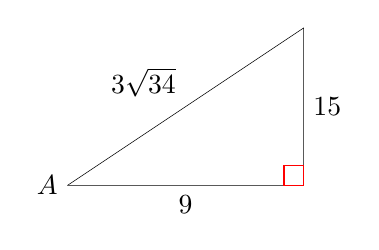
\begin{tikzpicture}
    \tkzDefPoints{0/0/A, 3/0/C, 3/2/B}
    \tkzDrawPolygon(A,B,C)
    \tkzMarkRightAngle[color=red](A,C,B)
    \tkzLabelPoints[left](A)
    \tkzLabelSegment[below](A,C){9}
    \tkzLabelSegment[right](C,B){15}
    \tkzLabelSegment[above left](A,B){$3\sqrt{34}$}
    \end{tikzpicture}
\end{minipage}
\begin{minipage}{0.4\textwidth}
\begin{align*}
    \onslide<2->{\sin A &= \frac{15}{3\sqrt{34}}} \\[11pt]
    \onslide<3->{&=\frac{5}{\sqrt{34}}} \\[11pt]
    \onslide<4->{&= \frac{5}{\sqrt{34}}\cdot \frac{\sqrt{34}}{\sqrt{34}}}    \\[11pt]
    \onslide<5->{&=\frac{5\sqrt{34}}{34}}
\end{align*}
\end{minipage}
\end{frame}

\begin{frame}{Example 1c}
\begin{minipage}{0.4\textwidth}
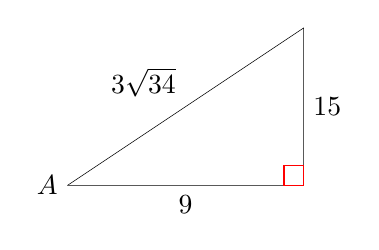
\begin{tikzpicture}
    \tkzDefPoints{0/0/A, 3/0/C, 3/2/B}
    \tkzDrawPolygon(A,B,C)
    \tkzMarkRightAngle[color=red](A,C,B)
    \tkzLabelPoints[left](A)
    \tkzLabelSegment[below](A,C){9}
    \tkzLabelSegment[right](C,B){15}
    \tkzLabelSegment[above left](A,B){$3\sqrt{34}$}
    \end{tikzpicture}
\end{minipage}
\begin{minipage}{0.4\textwidth}
\begin{align*}
    \onslide<2->{\cos A &= \frac{9}{3\sqrt{34}}} \\[11pt]
    \onslide<3->{&=\frac{3}{\sqrt{34}}} \\[11pt]
    \onslide<4->{&= \frac{3}{\sqrt{34}}\cdot \frac{\sqrt{34}}{\sqrt{34}}}    \\[11pt]
    \onslide<5->{&=\frac{3\sqrt{34}}{34}}
\end{align*}
\end{minipage}
\end{frame}

\begin{frame}{Example 1c}
\begin{minipage}{0.4\textwidth}
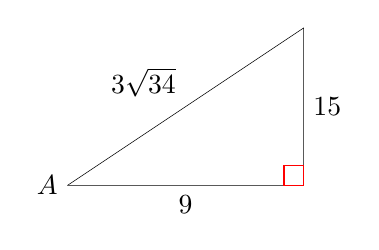
\begin{tikzpicture}
    \tkzDefPoints{0/0/A, 3/0/C, 3/2/B}
    \tkzDrawPolygon(A,B,C)
    \tkzMarkRightAngle[color=red](A,C,B)
    \tkzLabelPoints[left](A)
    \tkzLabelSegment[below](A,C){9}
    \tkzLabelSegment[right](C,B){15}
    \tkzLabelSegment[above left](A,B){$3\sqrt{34}$}
    \end{tikzpicture}
\end{minipage}
\begin{minipage}{0.4\textwidth}
\begin{align*}
    \onslide<2->{\tan A &= \frac{15}{9}} \\[11pt]
    \onslide<3->{&=\frac{5}{3}} \\
\end{align*}
\end{minipage}
\end{frame}

\begin{frame}{Other Trig Ratios}
In addition to the ``Big-3": sine, cosine, and tangent, there are three additional trigonometric ratios.    \nl    \pause

These ratios (\textit{cosecant}, \textit{secant}, and \textit{cotangent}) are the reciprocals of sine, cosine, and tangent, respectively.   \pause

\[
\csc A = \dfrac{\text{hypotenuse}}{\text{opposite}} \hspace{0.25in} \sec A = \dfrac{\text{hypotenuse}}{\text{adjacent}} \hspace{0.25in}  \cot A = \dfrac{\text{adjacent}}{\text{opposite}}    
\]
\end{frame}

\begin{frame}{Example 2a}
Write the exact ratios for cosecant, secant, and cotangent of angle $A$ for each of the following.  \nl
(a) \nl
\begin{minipage}{0.4\textwidth}
\begin{tikzpicture}
    \tkzDefPoints{0/0/A, 3/0/C, 3/2/B}
    \tkzDrawPolygon(A,B,C)
    \tkzMarkRightAngle[color=red](A,C,B)
    \tkzLabelPoints[left](A)
    \tkzLabelSegment[below](A,C){15}
    \tkzLabelSegment[right](C,B){8}
    \tkzLabelSegment[above,midway](A,B){17}
    \end{tikzpicture}
\end{minipage}
\begin{minipage}{0.4\textwidth}
\begin{align*}
    \onslide<2->{\csc A &= \frac{17}{8}} \\[11pt]
    \onslide<3->{\sec A &= \frac{17}{15}} \\[11pt]
    \onslide<4->{\cot A &= \frac{15}{8}}
\end{align*}
\end{minipage}
\end{frame}

\begin{frame}{Example 2b}
    (b) \nl
    \begin{minipage}{0.4\textwidth}
\begin{tikzpicture}
    \tkzDefPoints{0/0/A, 3/0/C, 3/2/B}
    \tkzDrawPolygon(A,B,C)
    \tkzMarkRightAngle[color=red](A,C,B)
    \tkzLabelPoints[left](A)
    \tkzLabelSegment[below](A,C){4}
    \tkzLabelSegment[right](C,B){3}
    \tkzLabelSegment[above,midway](A,B){5}
\end{tikzpicture}
\end{minipage}
\begin{minipage}{0.4\textwidth}
\begin{align*}
    \onslide<2->{\csc A &= \frac{5}{3}} \\[11pt]
    \onslide<3->{\sec A &= \frac{5}{4}} \\[11pt]
    \onslide<4->{\cot A &= \frac{4}{3}}
\end{align*}
\end{minipage}
\end{frame}

\begin{frame}{Example 2c}
    (c) \nl
\begin{minipage}{0.4\textwidth}
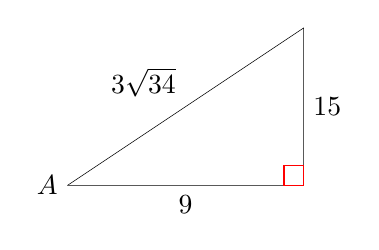
\begin{tikzpicture}
    \tkzDefPoints{0/0/A, 3/0/C, 3/2/B}
    \tkzDrawPolygon(A,B,C)
    \tkzMarkRightAngle[color=red](A,C,B)
    \tkzLabelPoints[left](A)
    \tkzLabelSegment[below](A,C){9}
    \tkzLabelSegment[right](C,B){15}
    \tkzLabelSegment[above left](A,B){$3\sqrt{34}$}
    \end{tikzpicture}
\end{minipage}
\begin{minipage}{0.4\textwidth}
\begin{align*}
    \onslide<2->{\csc A &= \frac{3\sqrt{34}}{15} = \frac{\sqrt{34}}{5}} \\[11pt]
    \onslide<3->{\sec A &= \frac{3\sqrt{34}}{9} = \frac{\sqrt{34}}{3}} \\[11pt]
    \onslide<4->{\cot A &= \frac{9}{15} = \frac{3}{5}}
\end{align*}
\end{minipage}    
\end{frame}

\section{Write the Exact Ratios for the Six Trigonometric Ratios of Special Angles}

\begin{frame}{45-45-90 Triangles}

45-45-90 triangles (also known as \textit{isosceles right triangles}) can be created by drawing a diagonal across a square:

\begin{center}
    \begin{tikzpicture}
    \tkzDefPoints{0/0/A, 3/0/B, 3/3/C, 0/3/D}
    \tkzDrawPolygon(A,B,C,D)
    \tkzMarkRightAngle[color=red](A,B,C)
    \tkzDrawSegment[dashed](A,C)
    \tkzLabelAngle[pos=0.75](B,A,C){$45^\circ$}
    \tkzLabelAngle[pos=0.75](B,C,A){$45^\circ$}
    \end{tikzpicture}
\end{center}

\end{frame} 

\begin{frame}{45-45-90 Triangles}
Since each side of a square is the same length, we can use whatever length we want. For simplicity, we will use a length of 1.  \nl \pause

The diagonal of the square can be found by using Pythagorean Theorem:  \pause

\begin{center}
    \begin{tikzpicture}
    \tkzDefPoints{0/0/A, 3/0/B, 3/3/C}
    \tkzDrawPolygon(A,B,C)
    \tkzMarkRightAngle[color=red](A,B,C)
    \tkzLabelAngle[pos=0.75](B,A,C){$45^\circ$}
    \tkzLabelAngle[pos=0.75](B,C,A){$45^\circ$}
    \tkzLabelSegment[right](B,C){1}
    \tkzLabelSegment[below](A,B){1}
    \tkzLabelSegment[above left, midway](A,C){$\sqrt{2}$}
    \end{tikzpicture}
\end{center}
\end{frame}

\begin{frame}{Example 3}
Find the exact values of the six trig ratios for $45^\circ$. \nl
\begin{minipage}{0.4\textwidth}
\begin{tikzpicture}
    \tkzDefPoints{0/0/A, 3/0/B, 3/3/C}
    \tkzDrawPolygon(A,B,C)
    \tkzMarkRightAngle[color=red](A,B,C)
    \tkzLabelAngle[pos=0.75](B,A,C){$45^\circ$}
    \tkzLabelAngle[pos=0.75](B,C,A){$45^\circ$}
    \tkzLabelSegment[right](B,C){1}
    \tkzLabelSegment[below](A,B){1}
    \tkzLabelSegment[above left, midway](A,C){$\sqrt{2}$}
    \end{tikzpicture}
\end{minipage}
\begin{minipage}{0.5\textwidth}
\begin{align*}
    \onslide<2->{\sin 45^\circ &= \frac{1}{\sqrt{2}}} \\[11pt]
    \onslide<3->{&= \frac{1}{\sqrt{2}}\frac{\sqrt{2}}{\sqrt{2}} = \frac{\sqrt{2}}{2}} \\[11pt]
    \onslide<4->{\cos45^\circ &= \frac{1}{\sqrt{2}} = \frac{\sqrt{2}}{2}} \\[11pt]
    \onslide<5->{\tan 45^\circ &= \frac{1}{1} = 1}
\end{align*}
\end{minipage}
\end{frame}

\begin{frame}{Example 3}
\begin{minipage}{0.4\textwidth}
\begin{tikzpicture}
    \tkzDefPoints{0/0/A, 3/0/B, 3/3/C}
    \tkzDrawPolygon(A,B,C)
    \tkzMarkRightAngle[color=red](A,B,C)
    \tkzLabelAngle[pos=0.75](B,A,C){$45^\circ$}
    \tkzLabelAngle[pos=0.75](B,C,A){$45^\circ$}
    \tkzLabelSegment[right](B,C){1}
    \tkzLabelSegment[below](A,B){1}
    \tkzLabelSegment[above left, midway](A,C){$\sqrt{2}$}
    \end{tikzpicture}
\end{minipage}
\begin{minipage}{0.5\textwidth}
\begin{align*}
    \onslide<2->{\csc 45^\circ &= \frac{\sqrt{2}}{1} = \sqrt{2}} \\[11pt]
    \onslide<3->{\sec45^\circ &= \frac{\sqrt{2}}{1} = \sqrt{2}} \\[11pt]
    \onslide<4->{\cot 45^\circ &= \frac{1}{1} = 1}    \\[11pt]
\end{align*}
\end{minipage}    
\onslide<5->{\emph{Note}: Your answers from the above example will be the same if you replace $45^\circ$ with $\frac{\pi}{4}$.}
\end{frame}

\begin{frame}{30-60-90 Triangles}
    We can create a 30-60-90 triangle by drawing an altitude in an equilateral triangle.

\begin{center}
    \begin{tikzpicture}
    \tkzDefPoints{0/0/A, 4/0/B}
    \tkzDefPoint(60:4){C}
    \tkzDrawPolygon(A,B,C)
    \tkzDefMidPoint(A,B)
        \tkzGetPoint{D}
    \tkzDrawSegment[dashed](D,C)
    \tkzMarkRightAngle[color=red](A,D,C)
    \tkzLabelAngle[pos=0.5](D,A,C){$60^\circ$}
    \tkzLabelAngle[pos=1](D,C,A){$30^\circ$}
    \end{tikzpicture}
\end{center}
\end{frame}

\begin{frame}{30-60-90 Triangles}
Recall that the altitude of an equilateral triangle bisects one of the sides.   \nl    \pause

Rather than use a length of 1 for the sides of the equilateral triangle, we will use a length of 2 (if only to avoid using fractions). \nl \pause

\begin{center}
    \begin{tikzpicture}
    \tkzDefPoints{0/0/A, 4/0/B}
    \tkzDefPoint(60:4){C}
    \tkzDrawPolygon(A,B,C)
    \tkzDefMidPoint(A,B)
        \tkzGetPoint{D}
    \tkzDrawSegment[dashed](D,C)
    \tkzMarkRightAngle[color=red](A,D,C)
    \tkzLabelAngle[pos=0.5](D,A,C){$60^\circ$}
    \tkzLabelAngle[pos=1](D,C,A){$30^\circ$}
    \tkzLabelSegment[below](A,D){1}
    \tkzLabelSegment[below](D,B){1}
    \tkzLabelSegment[midway, above left](A,C){2}
    \tkzLabelSegment[midway, above right](B,C){2}
    \end{tikzpicture}
\end{center}
\end{frame}

\begin{frame}{30-60-90 Triangles}
We can use the Pythagorean Theorem to find the length of the altitude, $\sqrt{3}$:

\begin{center}
    \begin{tikzpicture}
    \tkzDefPoints{0/0/A, 2/0/B}
    \tkzDefPoint(60:4){C}
    \tkzDrawPolygon(A,B,C)
    \tkzMarkRightAngle[color=red](A,B,C)
    \tkzLabelAngle[pos=0.5](B,A,C){$60^\circ$}
    \tkzLabelAngle(B,C,A){$30^\circ$}
    \tkzLabelSegment[below](A,B){1}
    \tkzLabelSegment[right](B,C){$\sqrt{3}$}
    \tkzLabelSegment[midway, above left](A,C){2}
    \end{tikzpicture}
\end{center}
\end{frame}

\begin{frame}{Example 4}
Find the exact values of the six trig ratios for $60^\circ$. \nl
\begin{minipage}{0.4\textwidth}
\begin{tikzpicture}
    \tkzDefPoints{0/0/A, 2/0/B}
    \tkzDefPoint(60:4){C}
    \tkzDrawPolygon(A,B,C)
    \tkzMarkRightAngle[color=red](A,B,C)
    \tkzLabelAngle[pos=0.5](B,A,C){$60^\circ$}
    \tkzLabelAngle(B,C,A){$30^\circ$}
    \tkzLabelSegment[below](A,B){1}
    \tkzLabelSegment[right](B,C){$\sqrt{3}$}
    \tkzLabelSegment[midway, above left](A,C){2}
    \end{tikzpicture}
\end{minipage}
\begin{minipage}{0.5\textwidth}
\begin{align*}
    \onslide<2->{\sin 60^\circ &= \frac{\sqrt{3}}{2}} \\[11pt]
    \onslide<3->{\cos 60^\circ &= \frac{1}{2}} \\[11pt]
    \onslide<4->{\tan 60^\circ &= \frac{\sqrt{3}}{1} = \sqrt{3}}
\end{align*}
\end{minipage}
\end{frame}

\begin{frame}{Example 4}
\begin{minipage}{0.4\textwidth}
\begin{tikzpicture}
    \tkzDefPoints{0/0/A, 2/0/B}
    \tkzDefPoint(60:4){C}
    \tkzDrawPolygon(A,B,C)
    \tkzMarkRightAngle[color=red](A,B,C)
    \tkzLabelAngle[pos=0.5](B,A,C){$60^\circ$}
    \tkzLabelAngle(B,C,A){$30^\circ$}
    \tkzLabelSegment[below](A,B){1}
    \tkzLabelSegment[right](B,C){$\sqrt{3}$}
    \tkzLabelSegment[midway, above left](A,C){2}
    \end{tikzpicture}
\end{minipage}
\begin{minipage}{0.5\textwidth}
\begin{align*}
    \onslide<2->{\csc 60^\circ &= \frac{2}{\sqrt{3}}} \\[11pt]
    \onslide<3->{&= \frac{2}{\sqrt{3}}\frac{\sqrt{3}}{\sqrt{3}} = \frac{2\sqrt{3}}{3}} \\[11pt]
    \onslide<4->{\sec 60^\circ &= \frac{2}{1} = 2} \\[11pt]
    \onslide<5->{\cot 60^\circ &= \frac{1}{\sqrt{3}}} \\[11pt]
    \onslide<6->{&= \frac{1}{\sqrt{3}}\frac{\sqrt{3}}{\sqrt{3}} = \frac{\sqrt{3}}{3}}
\end{align*}
\end{minipage}
\end{frame}

\begin{frame}{Example 5}
Find the exact values of the six trig ratios for $30^\circ$. \nl
\begin{minipage}{0.4\textwidth}
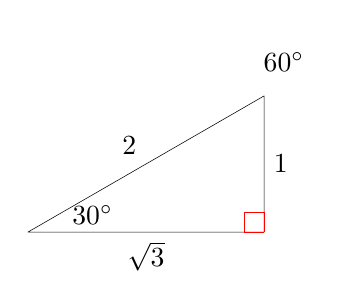
\begin{tikzpicture}
    \tkzDefPoints{0/0/A, 3/0/B, 3/1.73/C}
    \tkzDrawPolygon(A,B,C)
    \tkzMarkRightAngle[color=red](A,B,C)
    \tkzLabelAngle[pos=0.85](B,A,C){$30^\circ$}
    \tkzLabelAngle[pos=0.5](B,C,A){$60^\circ$}
    \tkzLabelSegment[below](A,B){$\sqrt{3}$}
    \tkzLabelSegment[right](B,C){1}
    \tkzLabelSegment[midway, above left](A,C){2}
    \end{tikzpicture}
\end{minipage}
\begin{minipage}{0.5\textwidth}
\begin{align*}
    \onslide<2->{\sin 30^\circ &= \frac{1}{2}} \\[11pt]
    \onslide<3->{\cos 30^\circ &= \frac{\sqrt{3}}{2}} \\[11pt]
    \onslide<4->{\tan 30^\circ &= \frac{1}{\sqrt{3}} = \frac{\sqrt{3}}{3}}
\end{align*}
\end{minipage}
\end{frame}

\begin{frame}{Example 5}
\begin{minipage}{0.4\textwidth}
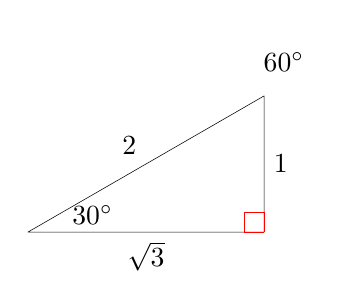
\begin{tikzpicture}
    \tkzDefPoints{0/0/A, 3/0/B, 3/1.73/C}
    \tkzDrawPolygon(A,B,C)
    \tkzMarkRightAngle[color=red](A,B,C)
    \tkzLabelAngle[pos=0.85](B,A,C){$30^\circ$}
    \tkzLabelAngle[pos=0.5](B,C,A){$60^\circ$}
    \tkzLabelSegment[below](A,B){$\sqrt{3}$}
    \tkzLabelSegment[right](B,C){1}
    \tkzLabelSegment[midway, above left](A,C){2}
    \end{tikzpicture}
\end{minipage}
\begin{minipage}{0.5\textwidth}
\begin{align*}
    \onslide<2->{\csc 30^\circ &= \frac{2}{1} = 2} \\[11pt]
    \onslide<3->{\sec 30^\circ &= \frac{2}{\sqrt{3}} = \frac{2\sqrt{3}}{3}} \\[11pt]
    \onslide<4->{\cot 30^\circ &= \frac{\sqrt{3}}{1} = \sqrt{3}}  \\[11pt]
\end{align*}
\end{minipage}    
\onslide<5->{Notice how $\sin 30^\circ = \cos 60^\circ$, $\tan 30^\circ = \cot 60^\circ$, etc. This is because these ratios are \alert{cofunctions}.}
\end{frame}

\end{document}
